\documentclass{article}
\usepackage[utf8]{inputenc}
\usepackage[margin=1in]{geometry}
\usepackage{amsmath}
\usepackage{hyperref}
\setlength{\parindent}{0em}
\setlength{\parskip}{0.5em}
\usepackage{graphicx} % Required for inserting images

\title{CTA200 2026 Assignment 3}
\author{Annalisa Teixeira}
\date{May 11th 2026}

\begin{document}

\maketitle

\section*{Question 1}

For this question, we will be considering points in the complex plane (given by $c = x + iy$), such that x, y $\in$ $(-2, 2)$.
From there, z is defined as:
\begin{equation}
    |z|^2 = \Re(z)^2 + \Im(z)^2
\end{equation} \label{z}
where 
\begin{equation}
    z_{i + 1} = z_i^2 + c
\end{equation} \label{iterate} 
with the initial condition $z_0 = 0$.

The aim of this question is to assess whether $|z|$ remains bounded or if it instead diverges to $\infty$.

I looped through the x and y values, computing the corresponding c value and iterating equation \ref{iterate}, until either the maximum number of iterations was exceeded or $|z|$ was found to be greater than 2, indicating divergence. c values that resulted in divergence of $|z|$ were marked as 'True', and the iteration of divergence is recorded. 
since x and y both span the same range, my code implicitly assumes the length of the x and y arrays to be the same. If x and y do not have the same length, the code can be easily adapted to account for this. If divergence has occurred before the first iteration, the iteration of divergence is recorded as '0'. 

An array of booleans indicating which c values lead to divergence is returned, along with a corresponding array that indicates the interval of divergence. These returns are used to construct the following two figures. 

\begin{figure}
    \centering
    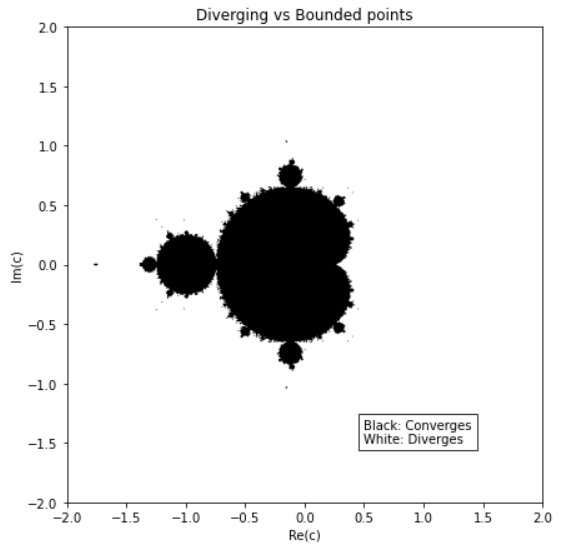
\includegraphics[width=0.5\linewidth]{Q1 div vs conv.png}
    \caption{Figure depicting the convergence or divergence of $|z|$ with respect to c, where $z_{i + 1} = z_i^2 + c$. Black indicates convergence, while white indicates divergence.}
    \label{fig:placeholder}
\end{figure}

\begin{figure}
    \centering
    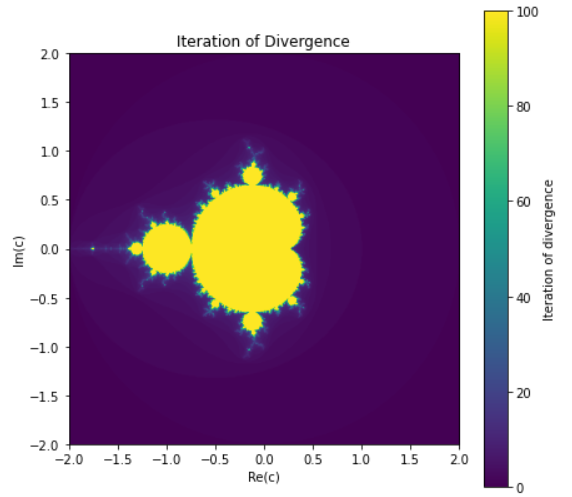
\includegraphics[width=0.5\linewidth]{Q1 it of div.png}
    \caption{Figure depicting the convergence or divergence of $|z|$ with respect to c, where $z_{i + 1} = z_i^2 + c$. Since the loop iterates 100 times, a value of yellow on the above figure indicates that the corresponding c does not lead to divergence.}
    \label{fig:placeholder}
\end{figure}

\section*{Question 2}

Lorenz' equations, established in \url{https://journals.ametsoc.org/view/journals/atsc/20/2/1520-0469_1963_020_0130_dnf_2_0_co_2.xml} are
\begin{eqnarray}
\dot X &=& -\sigma(X-Y)\\
\dot Y &=& rX -Y - XZ\\
\dot Z &=& -bZ + XY
\end{eqnarray} \label{ODES}
The non-linear terms in the second and third equations lead to complicated dynamics, resulting in unpredictable behaviour and great variation arising from small perturbations of the initial conditions. 

In his paper, Lorenz uses the following values for dimensionless parameters, which I adopted in my code:
\begin{eqnarray}
\mathrm{The\ Prandtl\ number:} \ \sigma = 10.0\\
\mathrm{The\ Rayleigh\ number:} \ r = 28.0 \\
\mathrm{Dimensionless \ length \ parameter:} \ b = \frac{8}{3}
\end{eqnarray}

Using solve\_ivp, I integrated equations \ref{ODES} from t = 0 to t = 60 (using dimensionless time units) with the initial conditions $W_0=[0., 1., 0.]$.

To reproduce Lorenz's Figure 1, I plotted the extracted solution of Y against $N = \frac{t}{\Delta t}$ where $\Delta t = 0.01$ (Fig. \ref{Q2.1}).
\begin{figure}
    \centering
    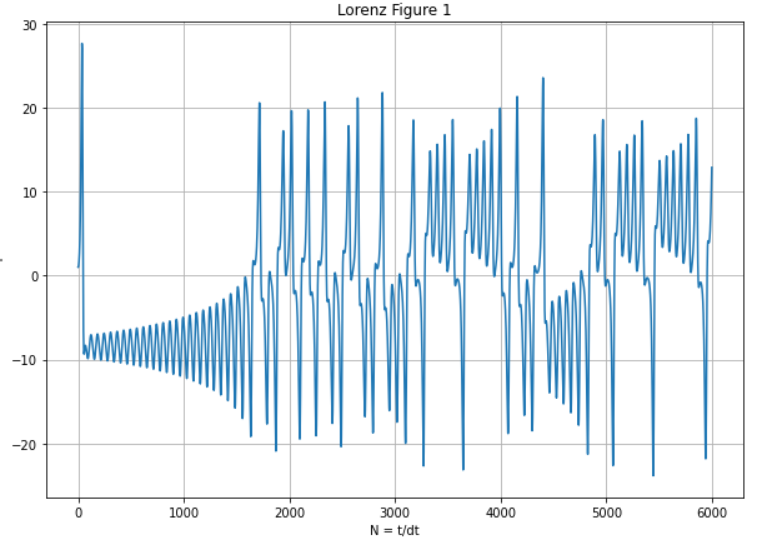
\includegraphics[width=0.5\linewidth]{Q2 fig 1.png}
    \caption{This figure displays the solution for Y plotted against $N = \frac{t}{\Delta t}$ where $\Delta t = 0.01$ over the time interval t = 0 to t = 60. The solution of Y was obtained through using solve\_ivp on \ref{ODES}. This is a recreation of Lorenz' figure 1. It should be noted that Lorenz deconstructs his figure into 3 figures, of 1000 iterations each.}
    \label{Q2.1}
\end{figure}

To reproduce Lorenz' Figure 2, I plotted the phase space for the X-Y and the Y-Z planes (Fig. \ref{Q2.2}, \ref{Q2.3}).

\begin{figure}
    \centering
    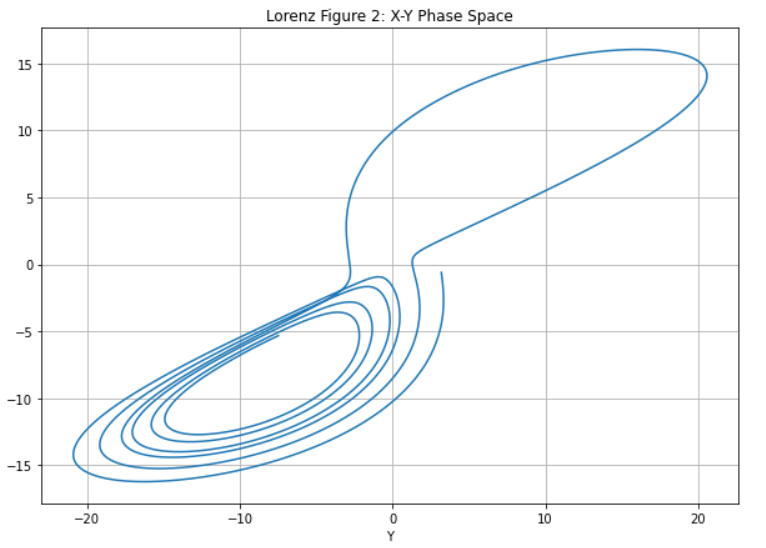
\includegraphics[width=0.5\linewidth]{Q2 fig 2 XY phase space.png}
    \caption{This figure depicts the X-Y plane in phase space, where the solutions to X and Y for times from t = 14 to t = 19 are obtained through solving equations \ref{ODES} using solve\_IVP.}
    \label{Q2.2}
\end{figure}

\begin{figure}
    \centering
    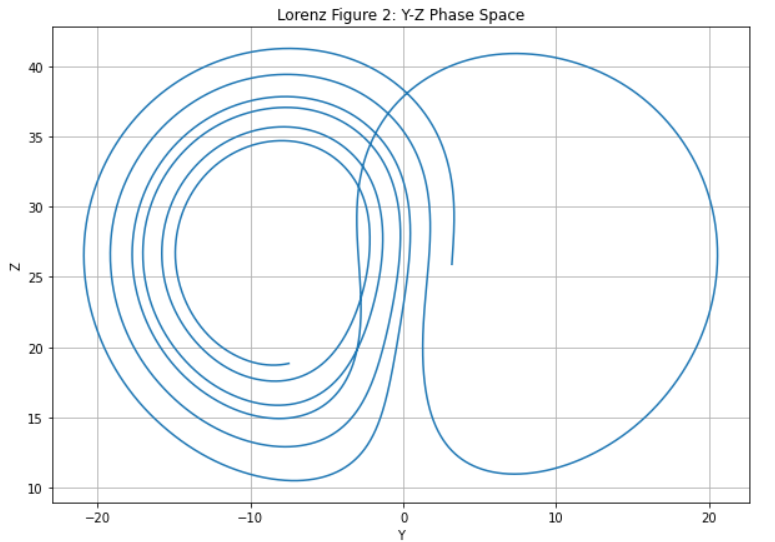
\includegraphics[width=0.5\linewidth]{Q2 fig 2 YZ phase space.png}
    \caption{This figure depicts the Y-Z plane in phase space, where the solutions to X and Y for times from t = 14 to t = 19 are obtained through solving equations \ref{ODES} using solve\_IVP.}
    \label{Q2.3}
\end{figure}

I then slightly perturbed the initial conditions, defining $W'_0 = W_0 + [0., 1.e-8, 0] = [0., 1.00000001, 0.]$. Using solve\_ivp I solved equations \ref{ODES} for initial conditions $W'$ and computed the distance between the trajectories predicted by $W'$ and $W$. I plotted this result (Fig. \ref{Q2.4}) on a semilog plot, where the distance is logged, while time remains plotted linearly. A straight line can be seen, indicating that a small deviation in the initial condition will result in divergence from the initial solution. Any error in the initial condition will grow exponentially.

\begin{figure}
    \centering
    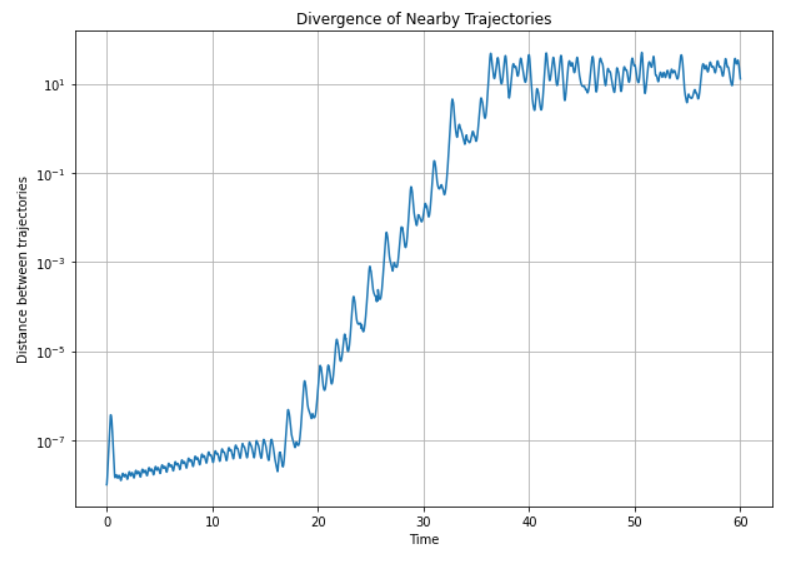
\includegraphics[width=0.5\linewidth]{Q2 p5.png}
    \caption{The distance between the solution trajectory predicted by initial conditions W = [0., 1.0, 0.] and W' = [0., 1.00000001, 0.]. This is a semilog plot, with linear time and logged distance. A straight line indicates exponential behaviour.}
    \label{Q2.4}
\end{figure}

\end{document}
